\documentclass[12pt,epsf,psfig,graphics]{article}             
\textwidth = 6.5in
\textheight = 9.05in
\topmargin 0.0in
\oddsidemargin 0.0in
\evensidemargin 0.0in

% set it so that subsubsections have numbers and they
% are displayed in the TOC (maybe hard to read, might want to disable)

\usepackage[T1]{fontenc}
\usepackage{mathptmx}

\usepackage{graphics}
\usepackage{pifont}
\setcounter{secnumdepth}{3}
\setcounter{tocdepth}{3}

% define widow protection 
        
\def\widow#1{\vskip #1\vbadness10000\penalty-200\vskip-#1}

% define a little section heading that doesn't go with any number

\def\littlesection#1{
\widow{2cm}
\vskip 0.5cm
\noindent{\bf #1}
\vskip 0.1cm
\noindent
}

% A paraphrase mode that makes it easy to see the stuff that shouldn't
% stay in for the final proposal

\newdimen\tmpdim
\long\def\paraphrase#1{{\parskip=0pt\hfil\break
\tmpdim=\hsize\advance\tmpdim by -15pt\noindent%
\hbox to \hsize
{\vrule\hskip 3pt\vrule\hfil\hbox to \tmpdim{\vbox{\hsize=\tmpdim
\def\par{\leavevmode\endgraf}
\obeyspaces \obeylines 
\let\par=\endgraf
\bf #1}}}}}

\renewcommand{\baselinestretch}{1.2}    % must go before the begin of doc
\newtheorem{principle}{Principle}
\newtheorem{definition}{Definition}
\newtheorem{define}{Definition}
% go with the way that CC sets the margins

\usepackage{listings}

\usepackage{color}

\definecolor{javared}{rgb}{0.6,0,0} % for strings
\definecolor{javagreen}{rgb}{0.25,0.5,0.35} % comments
\definecolor{javapurple}{rgb}{0.5,0,0.35} % keywords
\definecolor{javadocblue}{rgb}{0.25,0.35,0.75} % javadoc

\newcommand*\yes{\item[\Checkmark]}
\newcommand*\yesplus{\item[\Checkmark$^{+}$]}
\newcommand*\yesminus{\item[\Checkmark$^{-}$]}

\newcommand*\no{\item[\small{\XSolidBrush}]}

\begin{document}

\lstset{language=Java,
basicstyle=\ttfamily,
keywordstyle=\color{javapurple}\bfseries,
stringstyle=\color{javared},
commentstyle=\color{javagreen},
morecomment=[s][\color{javadocblue}]{/**}{*/},
%numbers=left,
numberstyle=\scriptsize\color{black},
stepnumber=1,
numbersep=7pt,
tabsize=4,
showspaces=false,
showstringspaces=false}

% handle widows appropriately
\def\widow#1{\vskip #1\vbadness10000\penalty-200\vskip-#1}

\begin{center}

CMPSC 440: Operating Systems\\
Examination One\\
%Saturday December 11, 2004 \\

\end{center}

\noindent
Answer the five questions that are listed on the following pages.  You must provide answers to these questions on a
separate sheet of paper.  Please develop responses that clearly express your ideas in the most succinct manner possible.
You are not permitted to complete this examination in conjunction with any of your classmates.  Furthermore, you cannot
consult any outside references during this examination.  If you have questions concerning the following problems, then
please visit my office during the examination period.  If you leave the classroom to take the exam, then you are
responsible for checking the white board for status updates.

%\mbox{} \newline
%\mbox{} \newline

\begin{enumerate}
  
\item ({\bf 10 Points}) The memory management unit (MMU) of an operating system controls what parts of a program are in
  memory and how those programs are accessed.  Answer the following questions about the MMU.
  
  \begin{enumerate}
          
  \item ({\bf 2 Points}) Many computers have both RAM and ROM.  What is the meaning of these two terms?  How does a
    computer operating system use both RAM and ROM?

  \item ({\bf 5 Points}) It is possible to divide up the computer's memory into address spaces.  What is an address
    space?  What does it mean if an address space is dynamically relocatable? How could the MMU use base and limit
    registers to support dynamic relocation?   

  \item ({\bf 3 Points}) Many operating systems support both virtual and physical memory.  After clearly defining both
    of these types of memory, please state which one is faster and explain why this is the case.
    
  \end{enumerate}
        
\newpage

% \begin{figure}[t]
%   \centering
%   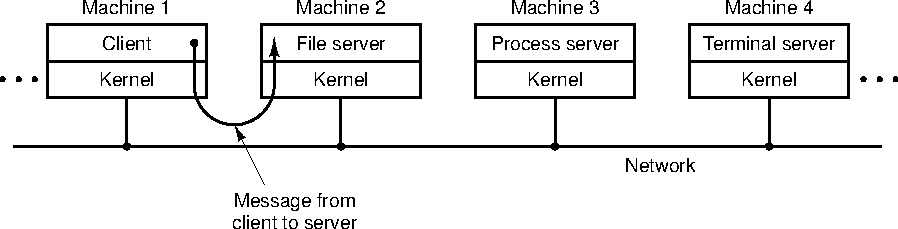
\includegraphics{fig1-27}
%   \caption{Client-Server Communication Involving the Client, a Server, and the Kernel.}
%   \label{fig:clientserver}
% \end{figure}
% 
\item ({\bf 10 Points}) There are many basic concepts that under gird the fundamentals of operating systems.  Answer the
  following questions about basic operating systems concepts.

  \begin{enumerate}
          
  \item ({\bf 4 Points}) A real-time operating system must schedule tasks to guarantee that a specified deadline will be
    met.  Draw a graph with a horizontal axis called ``time'', a vertical axis called ``utility'', and a vertical line
    at point $D$ on the horizontal axis.  Now, please draw a utility curve that represents the challenge associated with
    scheduling in a real-time operating system. Why did you draw this curve the way that you did?

  \item ({\bf 3 Points}) The shell of an operating system allows for the composition of processes using the pipe and
    filter architecture.  In the following code segment, what is the pipe? What is the filter? Why is this a good mode
    of interaction with the operating system?

    \begin{quote}
      {\tt cat file1 file2 file3 | sort > /dev/lp \&}
    \end{quote}

  \item ({\bf 3 Points}) Figure~\ref{fig:clientserver} furnishes an example of client-server communication with the
    support of the operating system kernel. Please outline all of the steps that must take place to support the
    communication between ``Machine 1'' and ``Machine 2''. 

  \end{enumerate}

  \newpage

\item ({\bf 10 Points}) Most, if not all, operating systems provide a kernel and many support virtualization. Answer the
  following questions about kernels and virtualization methods.

  \begin{enumerate}

    \item ({\bf 2 Points}) Most virtualization techniques distinguish between the guest operating system and the host
      operating system.  What is the meaning of these two terms? 

    \item ({\bf 3 Points}) How does the Java virtual machine support the standard of write-once run-anywhere? Your
      response to this question should use a properly labeled diagram.

    \item ({\bf 3 Points}) There are three representative types of operating systems kernels: microkernels, exokernels,
      and monolithic kernels. Using a properly labeled diagram for each definition, explain these types of kernels. What
      are their strengths and weaknesses?

    \item ({\bf 2 Points}) When implementing the process scheduler for the kernel, it is normally useful to ``separate
      policy and mechanism''.  What does this maxim mean? \mbox{Why is it important}?

  \end{enumerate}

  \newpage
  
\item ({\bf 10 Points}) The process is the main ``unit of work'' in an operating system.  Answer the following questions
  about processes and how they are managed by the operating system.

  \begin{enumerate}

    \item ({\bf 4 Points}) There are four events that can lead to the creation of a process. \mbox{What are they}?

    \item ({\bf 4 Points}) A process can be in one of three states: running, blocked, and ready. Using circles to
      represent each of these states and directed edges to denote transitions between these states, draw a process-state
      diagram. All states and edges must have labels.

    \item ({\bf 2 Points}) The operating system maintains a process table that stores information about each process
      that is currently executing on a computer. Using concrete examples whenever possible, please name and describe at
      least two of these fields.

  \end{enumerate}

  \newpage

  \begin{figure}[t]
    \centering
    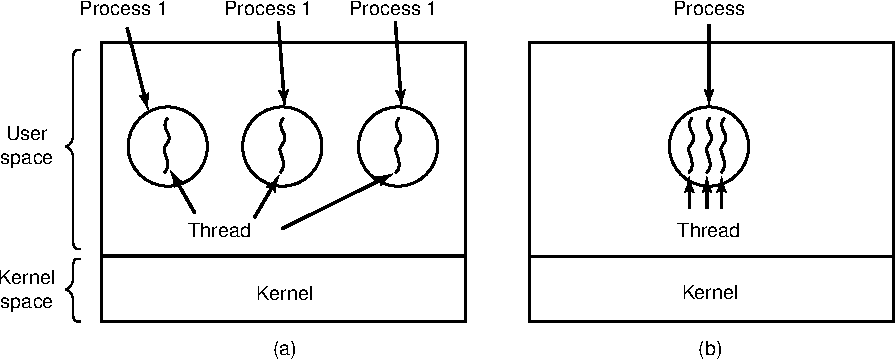
\includegraphics{fig2-11}
    \caption{Different Configurations of Processes and Threads.}
    \label{fig:pandt}
  \end{figure}


\item ({\bf 10 Points}) The operating system must provide primitives for scheduling threads and processes in a manner
  that avoids concurrency control problems. Answer the following questions about threads, processes, and concurrent
  execution.

\begin{enumerate}

  \item ({\bf 5 Points}) Figure~\ref{fig:pandt} shows two different canonical configurations of processes and threads. Answer the
    following questions about the trade-offs evident in this diagram.

    \begin{enumerate}

      \item Describe a scenario in which Figure~\ref{fig:pandt}(a) is:

        \begin{itemize}

          \item A good option for concurrent execution
          \item A poor option for concurrent execution

        \end{itemize}

      \item Describe a scenario in which Figure~\ref{fig:pandt}(b) is:

        \begin{itemize}

          \item A good option for concurrent execution
          \item A poor option for concurrent execution

        \end{itemize}

      \item If you were designing an operating system that could only support one of these models, which would you pick?
        Please justify your response to this question.

    \end{enumerate}

  \item ({\bf 5 Points}) Many kernel-mode and user-mode programs contain critical region(s) representing code
    segments that must be executed in mutual exclusion.  What is mutual exclusion? What are the four conditions that
    must be supported by any technique that aims to enforce mutual exclusion for a program's critical region?

\end{enumerate}

\end{enumerate}

\end{document}

